\scanpage{42}
Moyennant $C(Y)$, $C(X)$ équivaut à la condition
\[
\left|\begin{gathered}
\forall i\leq n-1,\quad\text{l'hom }\psi_\xi^i:H^i(Y)\longrightarrow H^i(X),\quad\text{inverse à gauche}\\
\text{naturel de }\varphi^i:H^i(X)\mathbin{-}H^i(Y),\quad\deleted{\text{\unsure{et}}}\quad\text{égal à }\Lambda_X\varphi_i\mid H^i(Y),\quad\text{est}\\
\text{induit par une classe algébrique.}
\end{gathered}\right.
\]
ou encore :
\[
\left|\quad\Lambda_X\varphi_*\text{ est algébrique}\right.
\]
\deleted{ou encore}\quad N.B. $\Lambda_X\varphi_*$ correspond à une classe de cohomologie
\inserted{$\text{dans }\sum H^{2(n-1)-i}(Y)\otimes H^i(X)=H^{2(n-\unsure{1|2})}(X\times Y)=H^{m-1}(X\times Y),\ m=\dim X\times\unsure{Y}$}
sur $X\times Y$, que nous \unsure{polarisons} par $\xi_X\otimes1+1\otimes\xi_Y$.
Or \deleted{$\unsure{\xi_X\otimes1+}$} $L_{X\times Y}(\Lambda_X\varphi_*)$ correspond à
\[
\begin{aligned}
\underbrace{\Lambda_X\varphi_*L_Y}_{\Lambda_XL_X\varphi_*}
 +\underbrace{L_X\Lambda_X\varphi_*}
 &=\deleted{\left(2\operatorname{id}-\sum_{\unsure{n|0}\leq i\leq2n}p_i^X\right)\varphi_*}\\
 &\inserted{=(\Lambda_XL_X+L_X\Lambda_X)\varphi_*}\\
 &=(\varphi_*\Lambda_Y\varphi^*+\operatorname{id}_X)\varphi_*.
\end{aligned}
\]
\deleted{$\unsure{\Lambda_XL_X\varphi_*}\quad\unsure{\varphi_*}\quad\unsure{2\operatorname{id}_X}$}
\figure{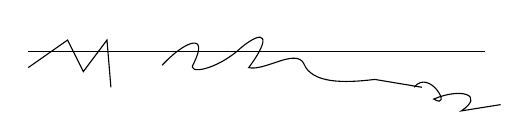
\begin{tikzpicture}[x=1cm,y=1cm]
\draw (0,.35)--(5.8,.35);
\draw (0,.15)--(.5,.5)--(.7,.1)--(1,.5)--(1.05,-.1);
\draw (1.7,.18) .. controls (2,.5) and (2.3,.6) .. (2.1,.2) .. controls (2,.05) and (2.4,.12) .. (2.7,.4) .. controls (3,.65) and (3.1,.55) .. (2.8,.15) .. controls (3,.1) and (3.4,.4) .. (3.5,.2) .. controls (3.6,-.05) and (4,-.05) .. (4.4,0) --(5,-.1);
\draw (4.9,-.1) .. controls (5.1,.15) and (5.4,-.4) .. (5.15,-.25) .. controls (5.5,-.1) and (5.8,-.2) .. (5.5,-.4) --(6,-.32);
\end{tikzpicture}}
(car $p_n^X\varphi_*=0$)

Donc est algébrique. Donc on trouve
\[
C(X)\Longleftrightarrow[C(Y)\text{ et }A^0(X\times Y)]
\]
puis de proche en proche
\[
C(X)\Longleftrightarrow\bigl(A^0(X\times Y)\text{ et }A^0(Y\times Z)\text{ et }A^0(Z\times T)\mathbin{-}\mathbin{-}\bigr)
\]
\deleted{$X\unsure{\sim}Y,\ \unsure{Y_\alpha}$}\quad
$X\supset Y\supset Z\supset T\mathbin{-}\mathbin{-}$ les uns sont \unsure{des sections} des autres, hyperplans non singuliers.

\figure{
\begin{tikzpicture}[x=.65cm,y=.65cm]
\node[rotate=45,text=blue!35] at (0.0,12.600000000000001){\unsure{Condor|Cordor|Concorde}};
\node[rotate=45,text=blue!35] at (2.1,12.600000000000001){\unsure{Condor|Cordor|Concorde}};
\node[rotate=45,text=blue!35] at (4.2,12.600000000000001){\unsure{Condor|Cordor|Concorde}};
\node[rotate=45,text=blue!35] at (6.300000000000001,12.600000000000001){\unsure{Condor|Cordor|Concorde}};
\node[rotate=45,text=blue!35] at (8.4,12.600000000000001){\unsure{Condor|Cordor|Concorde}};
\node[rotate=45,text=blue!35] at (10.5,12.600000000000001){\unsure{Condor|Cordor|Concorde}};
\node[rotate=45,text=blue!35] at (0.0,10.5){\unsure{Condor|Cordor|Concorde}};
\node[rotate=45,text=blue!35] at (2.1,10.5){\unsure{Condor|Cordor|Concorde}};
\node[rotate=45,text=blue!35] at (4.2,10.5){\unsure{Condor|Cordor|Concorde}};
\node[rotate=45,text=blue!35] at (6.300000000000001,10.5){\unsure{Condor|Cordor|Concorde}};
\node[rotate=45,text=blue!35] at (8.4,10.5){\unsure{Condor|Cordor|Concorde}};
\node[rotate=45,text=blue!35] at (10.5,10.5){\unsure{Condor|Cordor|Concorde}};
\node[rotate=45,text=blue!35] at (0.0,8.4){\unsure{Condor|Cordor|Concorde}};
\node[rotate=45,text=blue!35] at (2.1,8.4){\unsure{Condor|Cordor|Concorde}};
\node[rotate=45,text=blue!35] at (4.2,8.4){\unsure{Condor|Cordor|Concorde}};
\node[rotate=45,text=blue!35] at (6.300000000000001,8.4){\unsure{Condor|Cordor|Concorde}};
\node[rotate=45,text=blue!35] at (8.4,8.4){\unsure{Condor|Cordor|Concorde}};
\node[rotate=45,text=blue!35] at (10.5,8.4){\unsure{Condor|Cordor|Concorde}};
\node[rotate=45,text=blue!35] at (0.0,6.300000000000001){\unsure{Condor|Cordor|Concorde}};
\node[rotate=45,text=blue!35] at (2.1,6.300000000000001){\unsure{Condor|Cordor|Concorde}};
\node[rotate=45,text=blue!35] at (4.2,6.300000000000001){\unsure{Condor|Cordor|Concorde}};
\node[rotate=45,text=blue!35] at (6.300000000000001,6.300000000000001){\unsure{Condor|Cordor|Concorde}};
\node[rotate=45,text=blue!35] at (8.4,6.300000000000001){\unsure{Condor|Cordor|Concorde}};
\node[rotate=45,text=blue!35] at (10.5,6.300000000000001){\unsure{Condor|Cordor|Concorde}};
\node[rotate=45,text=blue!35] at (0.0,4.2){\unsure{Condor|Cordor|Concorde}};
\node[rotate=45,text=blue!35] at (2.1,4.2){\unsure{Condor|Cordor|Concorde}};
\node[rotate=45,text=blue!35] at (4.2,4.2){\unsure{Condor|Cordor|Concorde}};
\node[rotate=45,text=blue!35] at (6.300000000000001,4.2){\unsure{Condor|Cordor|Concorde}};
\node[rotate=45,text=blue!35] at (8.4,4.2){\unsure{Condor|Cordor|Concorde}};
\node[rotate=45,text=blue!35] at (10.5,4.2){\unsure{Condor|Cordor|Concorde}};
\node[rotate=45,text=blue!35] at (0.0,2.1){\unsure{Condor|Cordor|Concorde}};
\node[rotate=45,text=blue!35] at (2.1,2.1){\unsure{Condor|Cordor|Concorde}};
\node[rotate=45,text=blue!35] at (4.2,2.1){\unsure{Condor|Cordor|Concorde}};
\node[rotate=45,text=blue!35] at (6.300000000000001,2.1){\unsure{Condor|Cordor|Concorde}};
\node[rotate=45,text=blue!35] at (8.4,2.1){\unsure{Condor|Cordor|Concorde}};
\node[rotate=45,text=blue!35] at (10.5,2.1){\unsure{Condor|Cordor|Concorde}};
\node[rotate=45,text=blue!35] at (0.0,0.0){\unsure{Condor|Cordor|Concorde}};
\node[rotate=45,text=blue!35] at (2.1,0.0){\unsure{Condor|Cordor|Concorde}};
\node[rotate=45,text=blue!35] at (4.2,0.0){\unsure{Condor|Cordor|Concorde}};
\node[rotate=45,text=blue!35] at (6.300000000000001,0.0){\unsure{Condor|Cordor|Concorde}};
\node[rotate=45,text=blue!35] at (8.4,0.0){\unsure{Condor|Cordor|Concorde}};
\node[rotate=45,text=blue!35] at (10.5,0.0){\unsure{Condor|Cordor|Concorde}};
\end{tikzpicture}}
\mspage{41}
